\documentclass{article}
\usepackage[utf8]{inputenc}
\usepackage{listings}
\usepackage{xcolor}

\definecolor{codegreen}{rgb}{0,0.6,0}
\definecolor{codegray}{rgb}{0.5,0.5,0.5}
\definecolor{codepurple}{rgb}{0.58,0,0.82}
\definecolor{backcolour}{rgb}{0.95,0.95,0.92}
\usepackage{color}   %May be necessary if you want to color links
\usepackage{hyperref}
\usepackage{graphicx}
\graphicspath{ {./images/} }
\hypersetup{
    colorlinks=true, %set true if you want colored links
    linktoc=all,     %set to all if you want both sections and subsections linked
    linkcolor=black,  %choose some color if you want links to stand out
    urlcolor=blue,
}
\lstdefinestyle{mystyle}{
    backgroundcolor=\color{backcolour},   
    commentstyle=\color{codegreen},
    keywordstyle=\color{magenta},
    numberstyle=\tiny\color{codegray},
    stringstyle=\color{codepurple},
    basicstyle=\ttfamily\footnotesize,
    breakatwhitespace=false,         
    breaklines=true,                 
    captionpos=b,                    
    keepspaces=true,                 
    numbers=left,                    
    numbersep=5pt,                  
    showspaces=false,                
    showstringspaces=false,
    showtabs=false,                  
    tabsize=2
}

\lstset{style=mystyle}


\title{SMBUD}
\author{Filippo Lazzati, Martina Magliani, Christian Grasso, Sofia Martellozzo, Giacomo Lombardo}
%\date{October 2021}

\begin{document}
\thispagestyle{empty}
\begin{titlepage}
    \begin{center}
       %\vspace*{2cm}
       {\Huge \textbf{SMBUD}} %%Replace this with the Title of your research
       \vspace{0.5cm}
       \\
    \begin{LARGE}
        {Contact tracing app}
        \vspace{1.0cm}
        \\
        {\textit{Specification, Entity-Relationship model and Cypher code}}
           
\includegraphics[width=13cm]{polimi.png}
          \vspace{1.5cm}\\
                  Filippo Lazzati (10629918) - Martina Magliani (10682333) - Christian Grasso (10652464) - Sofia Martellozzo (10623060) - Giacomo Lombardo (10674987)\\
       {Year: 2021/2022}
    \end{LARGE}  
   \end{center}
\end{titlepage}
\newpage
\tableofcontents %this command creates an index
\newpage
\section{Problem specification}
The purpose of this project is to build an Information System that monitors and manages data about the COVID-19 pandemic for a specific country.
The first part of the project involves the design and development of a Contact Tracing system to monitor the viral diffusion. To be effective, a contact tracing system needs to store information about the contacts between citizens, possibly by keeping track of their relationships (e.g. family, work, etc...). This is key to keep the virus diffusion under control and allow authorities to quickly take action where the situation is critical.
To address the problem, we decided to store data in a graph database which allows us to easily manage and visualize the connections and to effectively retrieve significant information.
\section{Hypothesis}
The database is implemented under the following hypothesis:
\begin{itemize}
\item individuals can live together;
\item individuals who live together are constantly in contact with each other (contact tracing between them is not needed);
\item contacts between two individuals can be registered in two ways:
\begin{description}
\item through a contact tracing app (e.g. Immuni);
\item through public places’ registers (e.g. restaurants, theaters, etc…);
\end{description}
\item for each contact, time and place is stored (when possible); this means that usual contacts through the tracing app do not store the place, but only the time and duration of the contact;
\item if a person is tested positive, the system traces his/her direct contacts in the last 5 days;
\item if a person has a contact with a positive individual, he/she is notified to take a test: if the test results positive, his/her contacts are traced and notified too;
\item individuals who tested positive must take a test (booked by the system) 10 days after the first one. If it is negative they can end their isolation (recovered);
\item a test can be moved to another day;
\item people in isolation cannot go to other places but their house (for people with more houses, only 1 house is allowed);
\item the vaccine campaign has already started:
\begin{description}
\item for the non-vaccinated people testing is mandatory;
\item for the vaccinated people testing is not mandatory (but it is recommended);
\end{description}
\item one dose of vaccine suffices to obtain the green pass;
\item a test is inserted in the system when booked, but its result is \verb |UNKNOWN| until the test is made.
\item a person can own 1 or more devices;
\item every device can produce a \textit{CONTACT} relationship with another person.
\end{itemize}
\newpage
\section{Conceptual model}
The following is the Entity-Relationship (E-R) model of our database:\\ \\ \\
\vspace{1cm}
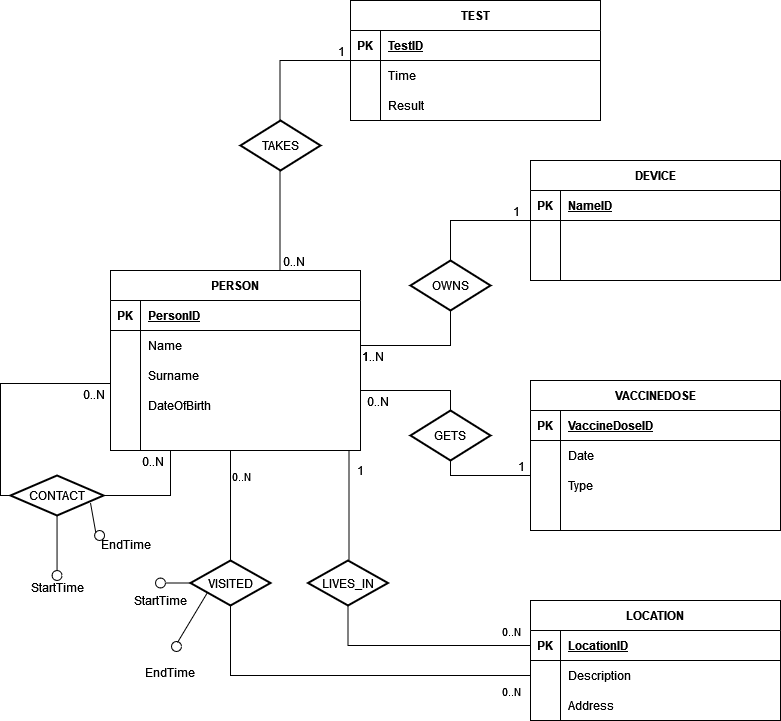
\includegraphics[scale=0.5]{images/e-r.png}
The Entity-Relationship model contains 5 different entities, that are related to each other through various relationships.
\begin{itemize}
    \item \textit{PERSON} represents the most important concept of the application, namely the user. Every \textit{PERSON} has a name, a surname and the date of birth. Of course the attributes of such entity could be enlarged, but as a sample dataset we have believed these three are enough;
    \item \textit{TEST} represents a test a person has to undergo when has been in contact with a positive (see the assumptions); a \textit{TEST} has 3 possible results, 'positive', 'negative' and 'unknown', where 'unknown' means that the test has been booked but the result is not known yet;
    \item \textit{DEVICE} represents a device owns by a person on which our contact tracing app is running; for the sake of simplicity it has only one attribute, the \textit{Name}, in addition to the Id;
    \item \textit{VACCINEDOSE} represents one single dose of vaccine received by a person; it has a date saying when it was administered and the type (brand) of the vaccine;
    \item \textit{LOCATION} represents either a place where a contact may occur or the home of a person. The attribute \textit{Address} specifies where it is located and \textit{Description} says its type (Home, Museum, ...).
\end{itemize}
Among these entities, some relations hold. In particular:
\begin{itemize}
    \item \textit{CONTACT} occurs between 2 different persons; it is recorded by the contact tracing app which specifies also the starting and the ending time;
    \item \textit{GETS} binds a person with its doses of vaccine;
    \item \textit{LIVES IN} specifies which person lives in which house. It is used to find people who live together;
    \item \textit{OWNS} simply relates a person to all his devices. It is a one-to-many relation;
    \item \textit{TAKES} binds a person with its tests;
    \item \textit{VISITED} is used to store data about when a certain person was in a certain place (ex.: museum, ...) and at which time, in order to find other people in the same place at the same time.
\end{itemize}
\newpage
\section{Sample dataset}
A sample dataset has been provided along with a file to initialize it. Such sample dataset has been built using some data found through the \href{https://datasetsearch.research.google.com}{Google dataset research} website at \href{https://www.kaggle.com/aleanfigeno/contact-tracing-application-sample-datasets/tasks}{this link}.This sample data has been modified and customised using some \verb|PHP| scripts.\\ In order to import it into your \verb |NEO4J| database, you have to put the files contained in the \href{https://github.com/filippolazzati/smbud/tree/main/graph\%20databases/sample\%20dataset\%20and\%20code/import}{import folder} of the project into the \textit{import} folder of the database in Neo4J. Then you can copy and paste the content of the \href{https://github.com/filippolazzati/smbud/blob/main/graph\%20databases/sample\%20dataset\%20and\%20code/inizialize\%20sample\%20dataset.cql}{inizialize sample dataset.cql} file into the Neo4J browser.In the following there is an explanation of such file.\\ \\
Since the sample dataset is given in \verb |CSV| files, you can exploit the \verb |LOAD| \verb |CSV| command to load the data (remember to put the files in the \verb |IMPORT| folder) :
\begin{enumerate}
    \item Clear the database: \lstinputlisting[language=SQL]{code/cmd0.txt}
    \item Load the locations: \lstinputlisting[language=SQL]{code/cmd1.txt}
    \item Load the persons: \lstinputlisting[language=SQL]{code/cmd2.txt}
    \item Create the \verb |LIVES| \verb |IN| relationship between users and locations:\lstinputlisting[language=SQL]{code/cmd3.txt}
    \item Create the \verb |VISITED| relationship between persons and locations:\lstinputlisting[language=SQL]{code/cmd4.txt}
    \item Load the devices: \lstinputlisting[language=SQL]{code/cmd5.txt}
    \item Create the \verb |OWNS| relationship between persons and devices:\lstinputlisting[language=SQL]{code/cmd6.txt}
    \item Load the tests' dates with the results (remember: a result can be any of \verb |POSITIVE|, \verb |NEGATIVE| or \verb |UNKNOWN|) :\lstinputlisting[language=SQL]{code/cmd7.txt}
    \item Create the \verb |TAKES| relationship between persons and tests:\lstinputlisting[language=SQL]{code/cmd8.txt}
    \item Load the contacts between people: \lstinputlisting[language=SQL]{code/cmd9.txt}
    \item Load the vaccines data about people:\lstinputlisting[language=SQL]{code/cmd10.txt}
    \item Create relationship \verb |GETS| between people and vaccine doses: \lstinputlisting[language=SQL]{code/cmd11.txt}
    \item Remove the attributes added only for creating the sample dataset: \lstinputlisting[language=SQL]{code/cmd12.txt}
\end{enumerate}
Now you have a working sample dataset on which you can try the queries of the following paragraph.
\newpage
\section{Queries and Commands}
The following queries and commands have been developed in order to provide an example of usage of the system for typical usage scenarios.
\subsection{Queries}
We have identified the following different queries.\\ It should be noticed that the 'xxx' ID has been used to select the considered person.
\begin{enumerate}
    \item \textbf{find people with one step of connection}.\\ This query can be written without the use of the \verb|UNION| construct in this way:
    \lstinputlisting[language=SQL]{code/query6.txt}
    \item \textbf{find people with two steps of connection}. \\In order to perform this query, we could easily repeat twice the previous one:
    \lstinputlisting[language=SQL]{code/query7.txt}
    However, in this way we are not able to take into consideration the timing constraints (see the assumptions). Therefore, another way (much longer) to perform the query is to first consider all the people who live with the considered person:
    \lstinputlisting[language=SQL]{code/query10.txt}
    next, we can consider all the people who our person 'xxx' met in the last 5 days:
    \lstinputlisting[language=SQL]{code/query11.txt}
    then we can consider all the people who our person 'xxx' has been in contact in the last 5 days according to our system:
    \lstinputlisting[language=SQL]{code/query12.txt}
    finally, we take all the possible combinations ($3^2 = 9$) of these three using the \verb|UNION| construct:
    \lstinputlisting[language=SQL]{code/query1end.txt}
    Clearly, this query is too long, and it is not able to take into account all the possible timing constraints; thus, the previous version shall be the preferred one.
    \item \textbf{find people with the Green Pass (i.e. vaccinated people or people with a negative test made in the last 2 days)}.\\ First, we have to consider all the people who underwent at least one vaccination (see the assumptions):
    \lstinputlisting[language=SQL]{code/query20.txt}
    next, we consider all the people who made a negative test in the last 2 days:
    \lstinputlisting[language=SQL]{code/query21.txt}
    finally, we compute the union of the 2:
    \lstinputlisting[language=SQL]{code/query22.txt}
    \item \textbf{find people who violated the isolation}.\\ For carrying out this query, the only information we can exploit is the data registered by restaurants, museums, ... According to the assumptions, a person must be at home from the day of a positive test until a negative test, 10 days later:
    \lstinputlisting[language=SQL]{code/query3.txt}
    \item \textbf{show the number of doses distributed for each brand of vaccine}.\\ We have to group all the vaccines and count them:
    \lstinputlisting[language=SQL]{code/query4.txt}
    \item \textbf{find people who are healed}. \\This is one of the simplest queries: we look for all the people with both a positive and a negative test, with the negative test made after the positive one:
    \lstinputlisting[language=SQL]{code/query5.txt}
    \item \textbf{return all the possible types of location}. \\The type of a Location can be directly accessed from a Location. The \verb|DISTINCT| construct should be used to avoid repeated results:
    \lstinputlisting[language=SQL]{code/query8.txt}
    \item \textbf{find all the people who were in place 'xxx' in date 2020-3-3}. \\The fields of a datetime, like the \textit{StartTime} of a \verb|VISITED| relationship can be accessed directly:
    \lstinputlisting[language=SQL]{code/query9.txt}
\end{enumerate}
\subsection{Commands}
We have identified the following \verb |INSERT| commands to show how the system works:
\begin{itemize}
    \item \textbf{insert a new person in the system}. \\I simply use the \verb|CREATE| construct to create such an instance; the only care I have to pay is for the use of the \textit{date}() function:
    \lstinputlisting[language=SQL]{code/command1.txt}
    \item \textbf{book a test for a person}.\\As it is specified in the assumptions, to book a test in our system a new \textit{Test} node has to be created with 'Unknown' \textit{Result}:
    \lstinputlisting[language=SQL]{code/command3.txt}
    \item \textbf{insert the result of a test}. \\We use the \verb|SET| construct to change the \textit{Result} attribute of the test:
    \lstinputlisting[language=SQL]{code/command4.txt}
    \item \textbf{modify the date of a test}. \\We use the \verb|SET| construct to change the \textit{Time} attribute of the test:
    \lstinputlisting[language=SQL]{code/command2.txt}
\end{itemize}
\section{User Interface}
\section{User guide}
\section{References and sources}
\begin{itemize}
    \item \href{https://datasetsearch.research.google.com}{Google Dataset Research}
    \item \href{https://www.kaggle.com/aleanfigeno/contact-tracing-application-sample-datasets/tasks}{Kaggle}
    \item \href{https://app.diagrams.net}{draw.io}
\end{itemize}

\end{document}
